\documentclass{article}
\usepackage[utf8]{inputenc}
\usepackage[frenchb]{babel}
\usepackage{graphicx}
\usepackage{color}

\title{STB v2 : Amélioration de la gestion des demandes en flux des utilisateurs}
\author{Juan PIRON}
\date{23 June 2017}
\begin{document}

\maketitle
\section{Objet du document}

Cette spécification définit les exigences relatives à une étude de la gestion en configuration des demandes de flux PGL via le logiciel CAPIRCA. Le besoin fonctionnel ayant était exprimé autour de 3 points :
\smallbreak 1/ adapter CAPIRCA pour la génération d’accès-liste ASA (similaires à celles des routeurs cisco).
\smallbreak 2/ Mettre en place un mécanisme de génération des règles et de leur gestion en configuration à partir des demandes de flux utilisateurs.
\smallbreak 3/ adapter les règles existantes pour les injecter dans le système CAPIRCA.

\maketitle
\section{Spécifications techniques actuelles}

La création et la gestion des demandes de flux ne ce fait pas directement en "CiscoASA" mais en passant par une interface de gestion développée par Cisco : ASDM (Adaptive Security Device Manager). Elle permet une gestion assez simplifiée et visuelle des ACLs. Mais ce "manager" ne permet pas un développement collaboratif, ni à distance. Il ne permet pas non plus de remonter aux demandes de flux initiales, qui ont permis de générer les règles en présence.

\maketitle
\section{Présentation générale de CAPIRCA}

Capirca est un outil conçu pour utiliser des définitions communes des réseaux, des services et des fichiers de règles (politiques) de haut niveau pour faciliter le développement et la manipulation des listes de contrôle d'accès réseau (ACL) pour diverses plates-formes. Il a été développé par Google pour un usage interne et est désormais open source.
Capirca simplifie le développement et la maintenance des filtres réseaux larges et complexes grâce à un seul et simple langage. Il fournit donc un langage de haut niveau facile à utiliser pour la définition des règles de sécurité réseau. Il permet la compilation des règles de sécurité en des filtres réseaux qui peuvent être appliqués à une variété de cibles (Cisco, Juniper, Iptables …).

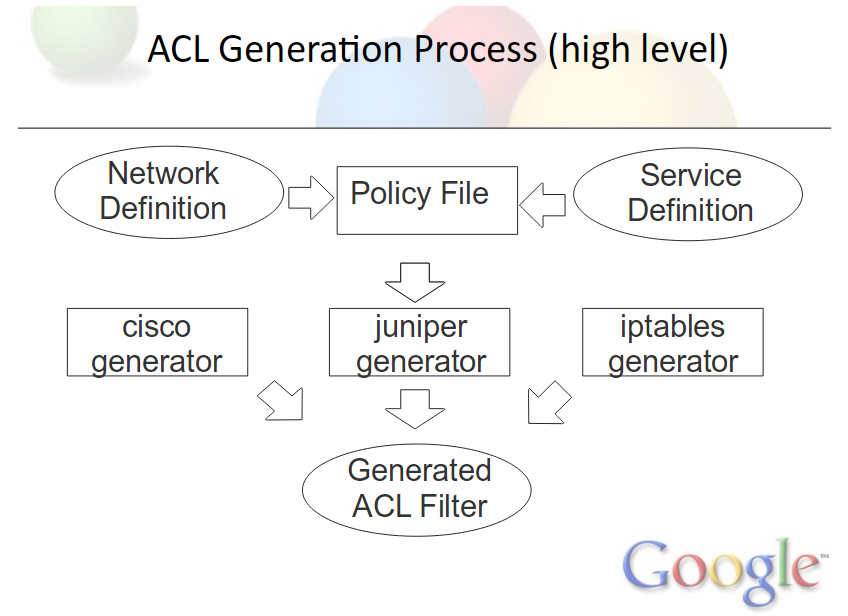
\includegraphics[scale=0.4]{capirca.png}

\maketitle
\section{Spécifications techniques envisagées}

Mettre en place un serveur git open source "Gobs". Créer dessus un repository sur lequel seul certaines personnes habilitées auront le droit d'accès et de modifications. En ce qui concerne la configuration actuelle des ACLs il y aurait deux manières distinctes de procéder. La première serait de récupérer simplement la "running-config" et les objets créés (uniquement "network" et "service").
Il suffit ensuite de créer un fichier ".pol" par demande de flux. En ce qui concerne la gestion de différences de version entre la "running-config" présente dans le repository et celle sur le "PGL" : avant toutes choses les "runnings" sont comparées pour vérifier que celle en présence est bien la dernière. Si ce n'est pas le cas la "running" est remplacée et tous nouveaux objets sont ajoutés.
La deuxième méthode serait de récupérer tous les objets présents dans la "running" même ceux non utilisables par capirca (icmp par exemple), et de les mettre dans une BDD. Par la suite, recréer le langage de haut niveau capirca correspondant aux différentes ACLs de la "running" (un fichier par interface).
Entre les deux méthodes, la seconde présente un intérêt pour son côté réintégration totale de la gestion et l'implémentation de la configuration du "PGL". En d'autres termes la seconde version court-circuite le "manager" (Cisco asdm). Or malgré le fait que le langage de haut niveau de capirca reste lisible, il ne le sera jamais autant que le "manager" pour les modifications de règles près existantes.
La première méthode permettrait donc une utilisation parallèle et complémentaire du "manager" et de Capirca/Gobs. Voici le résumé de façon schématique des deux méthodes envisageables :

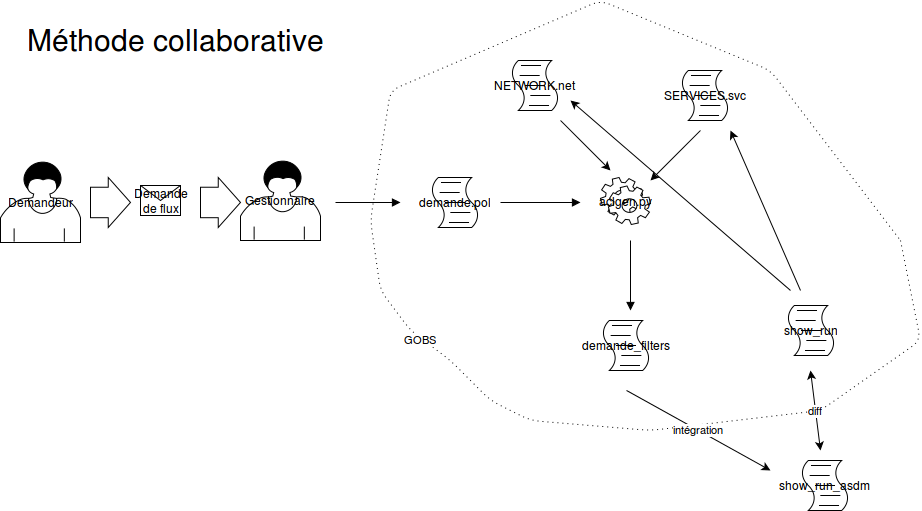
\includegraphics[scale=0.4]{collaborative.png}
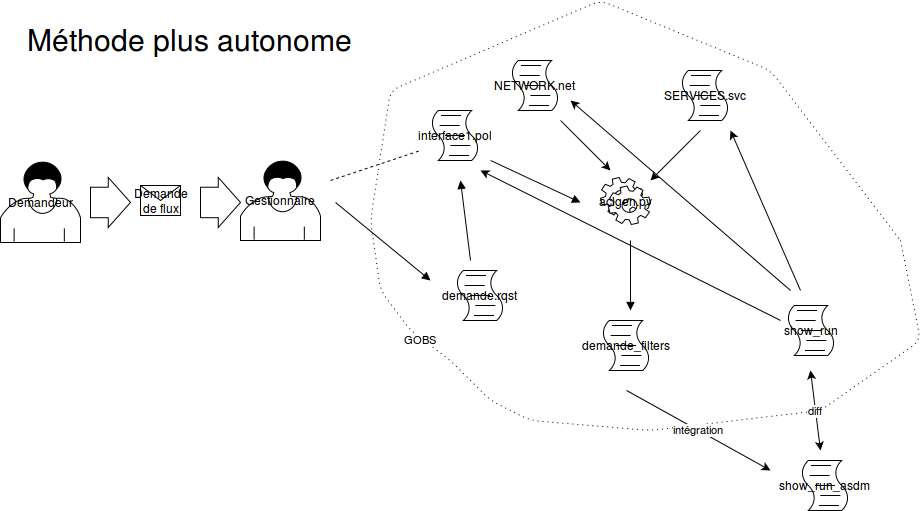
\includegraphics[scale=0.4]{autonome.png}
\end{document}
